\documentclass[a4paper,parskip=half,11pt]{scrartcl}

%%% Standardpakete
\usepackage[T1]{fontenc} 
\usepackage[utf8]{inputenc}
\usepackage[ngerman]{babel}
\usepackage{graphicx}

\usepackage{libertine} %Schriftart
\usepackage{tabularx} %fuer Tabellen
\usepackage{xcolor} %fuer Farben
\usepackage{amsmath} %fuer Mathematikmodus
%\usepackage[top=1cm]{geometry} %verringert Rand oben

\author{Trayracer: Oliver Kniejski, Steven Sobkowski, Marie Hennings}
\title{Bericht zum Szenegraph}

\begin{document}
 
\maketitle

\section*{Die Aufgabenstellung}
In der dieswöchigen Aufgabe geht es darum einen Szenegraph zu implementieren. Hierzu soll zunächst aus der Aufgabenstellung ein Klassendiagramm erstellt werden, um dies zu üben. Anschließend sollen drei neue Klassen(Node, Mat4x4, Transform) implementiert und die Geometrien angepassst werden. Zu guter Letzt müssen die abgebildeten Szenen ohne Vorgaben selbst nachgestellt werden.

\section*{Lösungsstrategien}
Dieses Mal wurden alle Aufgaben gemeinsam bearbeitet und gelöst.


\section*{Implementierung}
Die Aufgabe wurde anhand des selbstgemachten Klassendiagramms implementiert. Dabei wurde zuerst die Mat4x4-Klasse, dann die Transform-Klasse und anschließend die Node-Klasse erstellt und die Geometrien schließlich angepasst. 

\begin{figure}
\centering
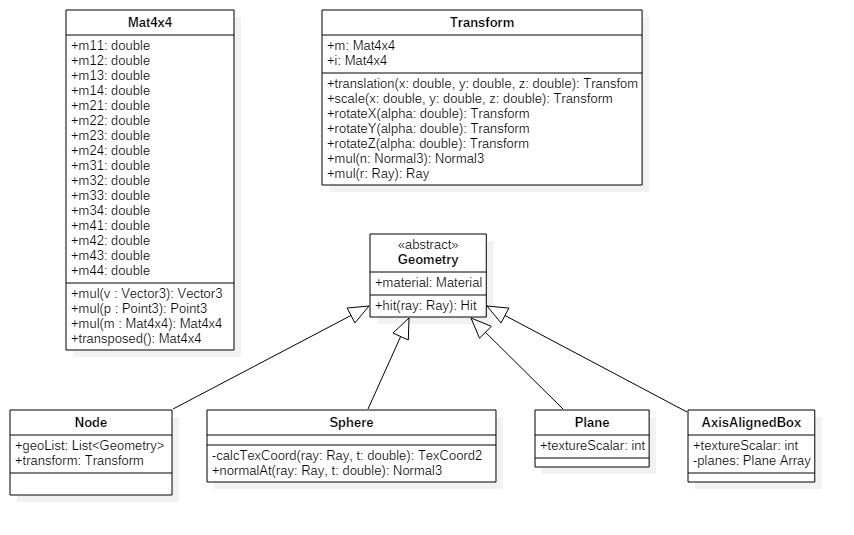
\includegraphics[width=\linewidth]{cg5}
\caption{Klassendiagramm}
\end{figure}


\section*{Besondere Probleme oder Schwierigkeiten bei der Bearbeitung}
Besondere Probleme gab es bei der Reihenfolge der Transformation, weil die Leserichtung zunächst nicht beachtet wurde. Die optionale Vergabe eines Materials in der Node-Klasse kostete Zeit und Hirnschmalz.

\section*{Zeitbedarf}
Der Zeitbedarf betrug ca. 9 Stunden.

\end{document}